\documentclass{article}
\usepackage{amsmath, amssymb}
\usepackage{array}
\usepackage{xcolor}
\usepackage{tikz}

\begin{document}

\section{Introduction}

Lecture 7 is about Kolmogorov Complexity.

\section{Berry's Paradox}

$S=$ ``The smallest positive integer that cannot be defined in under fifteen English words.'' This expression defines $S$ in under fifteen English words. Thus $S$ is not ``The smallest positive integer that cannot be defined in under fifteen English words.''

Solution: ``cannot be defined in under fifteen English words'' is not well defined. The one thing not well defined here is the word ``defined''. We need to formally define what we mean by ``defined''.

\section{Kolmogorov Complexity}

Which string is more random?
\[
101010101010101010101010101010
\]
or 
\[
001010101011111010101010100
\]
On one hand, once a string is written its not random any more. Also, both strings have the sam probability under uniform distribution. On the other hand, the first seems much less random. Why? Because there is a simple rule that explains it.

\subsection{Kolmogorov (1965)}
The longer it takes to describe/define a sequence of bits, the more random it is. If we can describe a string shortly, it is less random. If not, it is more random.

For a sequence of bits $x$, $K(x)=$ length in bits of shortest Java program that outputs $x$ and stops (the program has no input). $K(x)$ is a meausre for how much ``randomness'' there is in $x$. 

Intuition: $K(x)$ is the number of bits needed to describe/define $x$, but now the word ``defined'' is well defined.

\subsubsection{Example}
\[
101010101010101010
\]
versus
\[
100101110101010101
\]
The first string has a much ... and I missed it.

\subsection{Why Java?}

All programming languages are equivalent. $K(x)$ is not very sensitive to the programming language being used. If $K'(x)$ is Kolmogorov Complexity, is using a different language:
\[
K'(x) = K(x) \pm \mathcal{O}(1)
\]
We can think of Java as a Universal Turning Machine.

\subsubsection{Example}
\[
101010101010101010
\]
is repeat $n$ times. Here $n=10$. The Kolmogorov Complexity is $\leq\log n + \mathcal{O}(1)$, considered to be a small Kolmogorov Complexity. In generally, we usually ignore $\mathcal{O}(\log n)$  terms.

\subsubsection{Another example}

First $n$ binary digits of $\pi$. The Kolmogorov Complexity is  $\leq\log n + \mathcal{O}(1)$ (as there is a constant length program to output the digits of $\pi$, we just have to tell it how many digits we want).

\subsection{Upper Bound}

For any $x$ of length $n$,
\[
K(x) \leq n + \mathcal{O}(1)
\]
For almost all $x$ of length $n$,
\[
K(x)\approx n
\]
The argument is a counting argument.
\begin{itemize}
    \item Number of sequences of length $n$ is $2^n$
    \item Number of Java programs of length at most $n-c$ is $\leq 2^{n-c}$
    \item So at most $2^{-c}$ fraction of sequences $x$ of length $n$ have $K(x)\leq n-c$
\end{itemize}
A random sequence usually has $K(x)\approx n$.

\section{Kolmogorov Complexity vs Entropy}

$H(X)$ considers a random variable $X$ while $K(x)$ considers a fixed sequence $x$. Nevertheless, many intuitions are the same. Both measure the amount of uncertainty or randomness in $X$. Both measure the number of bits that take to describe $X$. Both measure how well we can compress $X$.

\subsection{Example}

Suppose $X=\left(X_1,\ldots,X_n\right)$ where they are i.i.d., then with high probability 
\[
K(X) \approx H(X)
\]
Example: Independent coin flips with probability $0.7$ for $1$ and $0.3$ for $0$. With high probability, we get a sequence with Kolmogorov complexity $\approx n\cdot \operatorname{H}(0.7,0.3)$

The two notions agree!

\subsection{Proof Sketch}

By Shannon's Source Coding Theorem, we know that there is a compression algorithm that compresses $X_1,\ldots,X_n$ to a string of length $\approx n\cdot H(X_i)$, such that from the string $X_1,\ldots,X_n$ can be retrieved with high probability.

The string plus the decoding algorithm show that with high probability,
\[
K(X) \leq n\cdot \left(H(X_i) + \delta\right)
\]

\subsection{Lower bound on $K(X)$}

By the Asymptotic Equipartition Theorem, we know that there are around $2^{n\cdot H(X_i)}$ typical sequences. On the other hand, the number of programs of length $\leq n \cdot \left(H(X_i) -\delta\right)$ is $\leq 2^{n \cdot \left(H(X_i) -\delta\right)}$. Thus with high probability
\[
K(X) \leq n \cdot \left(H(X_i) -\delta\right)
\]

\section{Conditional Kolmogorov complexity}

For two sequences of bits $x,y$ (possibly of different lengths), $K(x\mid y)=$ Kolmogorov Complexity of $x$ conditioned on $y$ equals length in bits of shortest Java program than on input $y$ outputs $x$ and stops.

Intuition: $K(x\mid y)$ is the number of bits needed to describe $x$ after seeing $y$.

\subsection{Chain Rule}
\[
K(x,y) = K(y) + K(x\mid y) + \mathcal{O}\left(\log n\right)
\]
where $n$ is the maximum length of $x$ and length of $y$. Equalities hold up to $\mathcal{O}\left(\log n\right)$ terms and is considered to be negligible.

Note that $K(x,y)$ means $x$ concatenated with $y$.

\section{Kolmogorov Complexity as a Universal Compression}

$K(x)$ can also be viewed as the length of the best compression of $x$. If we have a program of length $K(x)$ bits that outputs $x$, we have compressed $x$ to $K(x)$ bits.

\subsection{Kolmogorov Complexity as a Measure for Information}

$K(x)$ also measures the amount of information in $x$.

\subsection{Example}

The human genome is $3\cdot 10^9$ bases $A,G,C,T$ which equals $6\cdot 10^9$ bits, only! This is much smaller than the number of Neurons in our brain.

But the information that it contains is even smaller because the code an be compressed. The relevant number is the Kolmogorov Complexity of the code. No one knows what it is.

\section{Applications}

\subsection{There are Infinitely Many Primes}

Assume for a contradiction that there are only a finite number of primes $p_1,\ldots,p_m$ for some constant $m$.

Let $x$ be an integer of length $n$ bits. Then $x=\prod_{i=1}^{m}p_i^{d_i}$, where $d_1,\ldots,d_m\leq n$ (each $d_i$ is of length $\leq \log n$ bits).

Thus, $x$ can be described by giving $m$ numbers of length $\log n$ bits each. Thus,
\[
K(x)\leq \mathcal{O}(m\cdot \log n) = \mathcal{O}(\log n)
\]
in contradiction to the fact that with high probability $K(x) \geq n-10$. The proof can also give a lower bound on the density of prime numbers.

\section{Is Kolmogorov Complexity Computable?}

Given $x$, we can give better and better upper bound on $K(x)$ by giving programs that output $x$ and stop. Can we compute $K(x)$? Is there an alogrithm that on input $x$ outputs $K(x)$?

Attempt: Given $x$, enumerate over all programs, by lexicographic order, and find the first (and hence shortest) that output $x$.

Problem: The halting problem! There is no way to know if the machine will run forever, or stop and output $x$. In other words, there is no way to know if a program will output $x$ or not. 

\subsection{Kolmogorov Complexity is Incomputable}

Kolmogorov complexity has had theoretical impact, but very little practical output. The reason is that it is incomputable.

Assume for a contradiction that $K(x)$ is computable by a program of length $C$. Let
\[
C' = C + \log C + 10000
\]
Define $S$ as the smallest positive integer $x$ such that $K(x)\geq C'$. $S$ can be computed by the following program:
\begin{itemize}
    \item $x := 0$
    \item while $K(x) < C'$ do $x:=x +1$
    \item output $x$
\end{itemize}
The length of this program is smaller ($<$) than $C'$, thus $K(S) < C'$. This is a contradiction since, by definition of $S$, $K(S)\geq C'$.

\section{Back to Berry's Paradox}

$S$ equals the smallest positive integer that cannot be defined in under fifteen English words. The problem is with the word ``defined''. We need to formally define what we mean by ``defined''. We can try $S$ equals the smallest positive integer $x$, such that $K(x)\geq 10000$. But there is no program that outputs $S$, as $K(x)$ is incomputable. Paradox is resolved.

\section{Explicit Examples for Strings with High $K(x)$?}
Can we give an explicit (not random) example for a string $x$ with high Komolgorov Complexity? No!

\textbf{Theorem}: There exists a constant $C$ such that for any $x$, the statement $K(x)\geq C$ is unprovable. ($C$ depends on the mathematical theory in which we work, like ZFC, Peano Arithmetic, etc.)

Thus for most strings $x$ of length $>C+1$, we have $K(x)\leq C$, but we cannot prove it even for one string (of any length).

\textbf{Godels First Incompleteness Theorem (1931)}: For any (rich enough, consistent) mathematical theory, there exist statements that cannot be proved or disproved within the theory. 

$K(x)\geq C$ is an example for a statement that cannot be proved and for most strings is true so cannot be disproved.

\subsection{Proof}

For every $C$, define the program $T_C$:
\begin{enumerate}
    \item $y := 0$
    \item while $y$ is not a proof for a statement $K(x)\geq C$ do $y:= y +1$
    \item output the $x$ such that $y$ is a proof for the statement $K(x) \geq C$
\end{enumerate}
The program tries all possible proofs $y$ one by one, in lexicographic order, and checks if it proves a theorem for the from $K(x)\geq C$. It outputs the $x$ that corresponds to the first such proof, if exists (otherwise the program doesn't stop).

If the program stops and outputs $x$, what can we say about $K(x)$?

The length of $T_C$ is $\log C + D$, for some constant $D$. Thus 
\[
K(x) < \log C + D < C
\]
when $C$ is sufficiently large.

Contradiction! This is a contradiction since the program only outputs $x$, such that, $K(x)\geq C$. This is a contradiction to the assumption that the program stops and outputs $x$. Hence, the program never stops and $K(x)\geq C$ is unprovable.
% ---- Addendum: paste after \subsection{Proof} in the Kolmogorov complexity notes ----

\subsection{Addendum: Unpacking the Proof}

\subsubsection{Where does $x$ come from?}

The string $x$ is \emph{not} an input to $T_C$, and it is not written anywhere in the code of $T_C$. It is extracted from the proof that the program finds.

In a formal theory (ZFC, PA, \ldots), a proof is a finite string: a sequence of formulas, each of which is an axiom or follows from earlier formulas by an inference rule. The last formula is the theorem being proved. Since proofs are finite strings, $T_C$ can enumerate them $y = 0, 1, 2, \ldots$ and, for each $y$, mechanically check:
\begin{enumerate}
    \item Is $y$ a valid proof?
    \item Is its final line of the form ``$K(x)\geq C$'' (for the $C$ hardcoded in $T_C$)?
\end{enumerate}
A statement of this form contains the string $x$ explicitly, for example
\[
K(0110100111010110\cdots)\geq 1000000,
\]
so the program simply reads off the string inside $K(\cdot)$ and outputs it. The program does not \emph{choose} $x$: it outputs whatever string appears in the first such proof. Nobody knows in advance which $x$ that will be (or whether $T_C$ halts at all).

\subsubsection{Why is $|T_C| = \log C + D$?}

The only things written into $T_C$ are:
\begin{itemize}
    \item The number $C$, which takes $\approx \log C$ bits to write in binary. This is the only part that depends on $C$.
    \item Everything else: the enumeration loop, the proof checker for the theory (including its axioms), and the code that extracts $x$ from the final line. This is a fixed constant $D$ that depends on the theory, but \emph{not} on $C$ and \emph{not} on $x$.
\end{itemize}
If $x$ were hardcoded into $T_C$, the program would have length $\approx |x|$ and there would be no contradiction. The whole point is that $x$ is found by search, so it costs nothing in the description length.

Since $D$ does not depend on $C$, we can first fix the theory (which fixes $D$) and then choose $C$ large enough that $\log C + D < C$.

\subsubsection{The argument, step by step}

Suppose $T_C$ halts and outputs $x$. Then:
\begin{enumerate}
    \item The theory proves $K(x)\geq C$.
    \item Assuming the theory is \textbf{sound} (it only proves true statements), $K(x)\geq C$ really holds.
    \item But $T_C$ is a program of length $\log C + D$ that outputs $x$, so
    \[
    K(x) \leq |T_C| = \log C + D < C.
    \]
\end{enumerate}
Steps 2 and 3 contradict each other. Hence $T_C$ never halts, which means the theory proves $K(x)\geq C$ for \emph{no} string $x$.

Note the soundness assumption in step 2: without it, the theory could ``prove'' false statements of the form $K(x)\geq C$, and there would be no contradiction.

\subsubsection{Remarks}

\begin{itemize}
    \item \textbf{Most strings do have $K(x)\geq C$.} There are fewer than $2^C$ programs of length less than $C$, so among the $2^n$ strings of length $n > C$, almost all satisfy $K(x)\geq C$. The statement is true for almost every long string, yet it cannot be proved for even a single specific one.
    \item \textbf{Corrections to the notes above.} ``For most strings $x$ of length $>C+1$, we have $K(x)\leq C$'' should read $K(x)\geq C$, and the final ``$K(x)\leq C$ is unprovable'' should read ``$K(x)\geq C$ is unprovable.''
    \item This result is known as \textbf{Chaitin's incompleteness theorem}. It gives a concrete family of true but unprovable statements, as promised by G\"odel's first incompleteness theorem.
\end{itemize}

\section{Unprovability Paradox}

$K(x) \geq C$ is unprovable. $K(x) < C$ is provable (when true)
\[
m = \lvert \left\{ x \text{ of length} \leq C : K(x) \geq C \right\} \rvert
\]
(that is strings of length $\leq C$, with $K(x)\geq C$). We proved $m\geq 1$ by a counting argument. We will prove $m\geq 2$.

\subsection{Proof}

... I missed it.

\subsection{We can prove $m\geq 3$}

... I missed it.

\subsection{Working our way up}

Working our way up, we get $m> 2^{C+1}$, which is a contradiction!

Contradiction to what??? We had no assumption! It is an implicit assumption. It is a contradiction to an implicit assumption that the consistency of the theory can be proved.

\textbf{Godels Second Incompleteness Theorem}: For any (rich enough, consistent) mathematical theory, the consistency of the theory itself cannot be proved or disproved within the theory.

\section{Universal Compression}

We proved theorems that show that in some cases a random variable can be compressed to its entropy. What if the distribution of the random variable is not known? Or maybe the random variable doesn't even exist. We just have a file of, say, bits, that we want to compress. 

Lempel-Ziv is a very well known and widely used algorithm for compressing files, that has excellent performance both theoretically and practically.

\subsection{Lempel-Ziv Code}

Given a string of bits 
\[
1111110101111011011011100111111111111010
\]
Partition it into words, such that, each word is the shortest one that hasn't appeared before
\[
1,11,111,0,10,1111,01,101,1011,100,11111,111111,1010
\]
Index the words. Encode each word (of length $k$) by the index corresponding to the words of its $k-1$ prefix, plus the additional bit

\begin{tabular}{c|c|c|c|c|c|c|c|c|c|c|c|c}
1 & 11 & 111 & 0 & 10 & 1111 & 01 & 101 & 1011 & 100 & 11111 & 111111 & 1010 \\
1 & 2 & 3 & 4 & 5 & 6 & 7 & 8 & 9 & 10 & 11 & 12 & 13 \\
0;\,1 & 1;\,1 & 2;\,1 & 0;\,0 & 1;\,0 & 3;\,1 & 4;\,1 & 5;\,1 & 8;\,1 & 5;\,0 & 6;\,1 & 11;\,1 & 8;\,0
\end{tabular}

% Preamble: \usepackage{tikz}
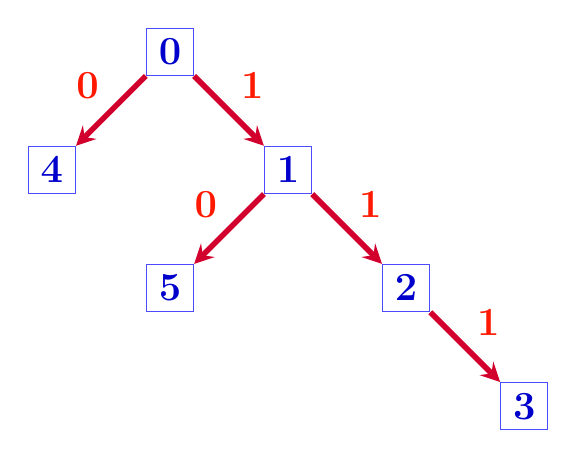
\begin{tikzpicture}[
    every node/.style={font=\bfseries\Large},
    box/.style={draw=blue!70, text=blue!80!black, inner sep=2pt, minimum size=0.6cm},
    edge/.style={->, >=stealth, line width=2pt, draw=purple!70!red},
    lbl/.style={text=red!80!orange}
]
  % Nodes
  \node[box] (n0) at (0,0)       {0};
  \node[box] (n4) at (-1.5,-1.5) {4};
  \node[box] (n1) at (1.5,-1.5)  {1};
  \node[box] (n5) at (0,-3)      {5};
  \node[box] (n2) at (3,-3)      {2};
  \node[box] (n3) at (4.5,-4.5)  {3};

  % Edges with labels
  \draw[edge] (n0) -- node[lbl, above left]  {0} (n4);
  \draw[edge] (n0) -- node[lbl, above right] {1} (n1);
  \draw[edge] (n1) -- node[lbl, above left]  {0} (n5);
  \draw[edge] (n1) -- node[lbl, above right] {1} (n2);
  \draw[edge] (n2) -- node[lbl, above right] {1} (n3);
\end{tikzpicture}

The idea is that in non-random sequences, there are lost of repetitions. From the encoding, it's easy to decode and get the original message.

\section{Entropy Rate}

A source is an infinite sequence of random variables $X_1,X_2,X_3,\ldots$

Consider 
\[
h=\lim_{k\to \infty} \frac{1}{k}\operatorname{H}\left(X_1,\ldots, X_k\right)
\]
When the limit exists, $h$ is called the entropy rate of the source. The limit doesn't always exist, but it does exist for wide classes of sources. When the limit exists, and $n\to \infty$, Lempel-Ziv algorithm compresses a sequence of length $n$ to a sequence of length $h\cdot n+\mathcal{o}(n)$ with high probability. This is the best that we could hope for.

\end{document}